%%%%%%%%%%%%%%%%%%%%%%%%%%%%%%%%%%%%%%%%%
% baposter Landscape Poster
% LaTeX Template
% Version 1.0 (11/06/13)
%
% baposter Class Created by:
% Brian Amberg (baposter@brian-amberg.de)
%
% This template has been downloaded from:
% http://www.LaTeXTemplates.com
%
% License:
% CC BY-NC-SA 3.0 (http://creativecommons.org/licenses/by-nc-sa/3.0/)
%
%%%%%%%%%%%%%%%%%%%%%%%%%%%%%%%%%%%%%%%%%

%----------------------------------------------------------------------------------------
%	PACKAGES AND OTHER DOCUMENT CONFIGURATIONS
%----------------------------------------------------------------------------------------

\documentclass[portrait,fontscale=0.40,paperwidth=30in, paperheight=40in,margin=1in]{baposter} % Adjust the font scale/size here
% 0.285
\usepackage{xcolor}
\usepackage{fancyhdr}
%\usepackage{tgschola} % or any other font package you like
\usepackage{setspace}
\usepackage{mathrsfs}
\usepackage{epsfig}
\usepackage{amssymb}
\usepackage{amsmath}
\usepackage{amsbsy}
\usepackage{bm}
\usepackage{grffile}
\usepackage{graphicx}
\usepackage{relsize}
\usepackage{amssymb}
\usepackage{relsize}
\usepackage[font=scriptsize]{caption}
\usepackage{subcaption}
\usepackage{float}
\usepackage{algpseudocode}
\usepackage{algorithm}
\usepackage{epstopdf}

\usepackage{amsmath, amsthm, amssymb, mathtools, thmtools, mathdots, tikz, pgfplots}
\mathtoolsset{showonlyrefs}



\newcommand{\eat}[1]{}




\usepackage[utf8]{inputenc}
\usepackage[english]{babel}

 \usepackage{amsthm}
\newtheorem{theorem}{Theorem}
\theoremstyle{definition}
\newtheorem{definition}{Definition}[section]

\theoremstyle{remark}
\newtheorem*{remark}{Remark}

%\newcommand{\m}[1]{\mathcal{#1}}
%\renewcommand{\b}[1]{\mathbb{#1}}
\DeclarePairedDelimiter{\parens}{(}{)}
\DeclarePairedDelimiter{\braces}{\{}{\}}
\DeclarePairedDelimiter{\brackets}{[}{]}
\DeclarePairedDelimiter{\abs}{|}{|}
\DeclarePairedDelimiter{\norm}{\|}{\|}
\DeclarePairedDelimiter{\inner}{\langle}{\rangle}
\DeclarePairedDelimiter{\ceil}{\lceil}{\rceil}
\DeclarePairedDelimiter{\floor}{\lfloor}{\rfloor}
\DeclareMathOperator*{\argmin}{\arg\!\min}
\DeclareMathOperator*{\argmax}{\arg\!\max}
\newcommand{\indep}{\mathop{\rotatebox[origin=c]{90}{$\models$}}}
%\newcommand{\notindep}{\mathop{\rotatebox[origin=c]{90}{$\models$}}}
%\DeclareMathOperator{\im}{im}
%\DeclareMathOperator{\Aut}{Aut}
%\DeclareMathOperator{\Inn}{Inn}
%\DeclareMathOperator{\lcm}{lcm}
%\DeclareMathOperator{\trace}{trace}
%\DeclareMathOperator{\Hom}{Hom}
%\DeclareMathOperator{\red}{red}
\newcommand{\op}[1]{\operatorname{#1}}
\renewcommand{\b}[1]{\boldsymbol{\mathbf{#1}}}
\renewcommand{\bar}[1]{\overline{#1}}
\renewcommand{\hat}[1]{\widehat{#1}}
\renewcommand{\tilde}[1]{\widetilde{#1}}
\newcommand{\E}{\mathbb{E}}
\renewcommand{\P}{\mathbb{P}}
\newcommand{\Var}{\op{Var}}
\newcommand{\Cov}{\op{Cov}}
\newcommand{\R}{\mathbb{R}}
\newcommand{\N}{\mathbb{N}}



\usepackage{graphicx} % Required for including images
%\graphicspath{{figures/}} % Directory in which figures are stored

\usepackage{amsmath} % For typesetting math
\usepackage{amssymb} % Adds new symbols to be used in math mode

\usepackage{booktabs} % Top and bottom rules for tables
\usepackage{enumitem} % Used to reduce itemize/enumerate spacing
\usepackage{palatino} % Use the Palatino font
\usepackage[font=small,labelfont=bf]{caption} % Required for specifying captions to tables and figures

\usepackage{multicol} % Required for multiple columns
\setlength{\columnsep}{1.0em} % Slightly increase the space between columns
\setlength{\columnseprule}{0mm} % No horizontal rule between columns

\usepackage{tikz} % Required for flow chart
\usetikzlibrary{shapes,arrows} % Tikz libraries required for the flow chart in the template

\newcommand{\compresslist}{ % Define a command to reduce spacing within itemize/enumerate environments, this is used right after \begin{itemize} or \begin{enumerate}
\setlength{\itemsep}{1pt}
\setlength{\parskip}{0pt}
\setlength{\parsep}{0pt}
}

\definecolor{lightblue}{rgb}{0.145,0.6666,1} % Defines the color used for content box headers

\begin{document}

\begin{poster}
{
headerborder=closed, % Adds a border around the header of content boxes
colspacing=1em, % Column spacing
bgColorOne=white, % Background color for the gradient on the left side of the poster
bgColorTwo=white, % Background color for the gradient on the right side of the poster
borderColor=lightblue, % Border color
headerColorOne=black, % Background color for the header in the content boxes (left side)
headerColorTwo=lightblue, % Background color for the header in the content boxes (right side)
headerFontColor=white, % Text color for the header text in the content boxes
boxColorOne=white, % Background color of the content boxes
textborder=roundedleft, % Format of the border around content boxes, can be: none, bars, coils, triangles, rectangle, rounded, roundedsmall, roundedright or faded
eyecatcher=true, % Set to false for ignoring the left logo in the title and move the title left
headerheight=0.1\textheight, % Height of the header
headershape=roundedright, % Specify the rounded corner in the content box headers, can be: rectangle, small-rounded, roundedright, roundedleft or rounded
headerfont=\large\bf\textsc, % Large, bold and sans serif font in the headers of content boxes
%textfont={\setlength{\parindent}{1.5em}}, % Uncomment for paragraph indentation
linewidth=2pt % Width of the border lines around content boxes
}
%----------------------------------------------------------------------------------------
%	TITLE SECTION
%----------------------------------------------------------------------------------------
%
{
%
\includegraphics[height=4em]{images/berkeley.png}
} % First university/lab logo on the left
{
{When Variational Auto-encoders meet Generative Adversarial Networks}
\vspace{0.5em}
} % Poster title
{\textsc{Jianbo Chen, Billy Fang, Cheng Ju
\hspace{12pt}
\textit{Departments of Statistics and Biostatistics, UC Berkeley}
\hspace{12pt} CS 294-129, Fall 2016
%\vspace{-2em}
}} % Author names and institution


%----------------------------------------------------------------------------------------
%	OBJECTIVES
%----------------------------------------------------------------------------------------


\headerbox{Problems}{name=Problem,column=0,row=0}{
\begin{itemize}\compresslist
    \item Various generative model of images.
    \item Various applications including semi-supervised learning.
\end{itemize}
}
\headerbox{Backgrounds and Objectives}{name=Background,column=0,below = Problem}{
\begin{itemize}\compresslist
    \item Variational auto-encoders (VAE) use variational inference to learn intractable posterior distributions.
    \item VAE's drawbacks: Images tend to be blurry.
    \item Generative adversarial networks (GAN) learn a generative model based on game theory.
    \item GAN's drawbacks: Difficult to train; No explicit representation of the generative distribution $p_g(x)$.
    \item Intermediate Objectives: Investigate various types of VAE models. % Mention that we put emphasis on VAE.
    \item Ultimate Goal: Combine VAE and GAN to get 'better' generative models.
\end{itemize}
%\vspace{0.3em} % When there are two boxes, some whitespace may need to be added if the one on the right has more content
}
%\headerbox{Data and Tools}{name=Data,column=0,below = Background}{
%\begin{itemize}\compresslist
%    \item Data: MNIST digits dataset and SVHN dataset
%    \item Tools: TensorFlow, GeForce GTX 770 GPU
%\end{itemize}
%}
%----------------------------------------------------------------------------------------
%	INTRODUCTION
%----------------------------------------------------------------------------------------

\headerbox{Variational auto-encoder}{name=VAE,column=0,below=Background}{
\textbf{Variational auto-encoder (VAE)} \cite{kingma2013auto}
\begin{itemize}\compresslist
    \item Latent variable model: $z \sim \mathcal{N}(0,I)$, $x \mid z \sim f(x;z,\theta)$ (e.g. Bernoulli)
    \item Variational inference: maximize lower bound on log likelihood
\end{itemize}
\[\log p(x) \ge \E_{z \sim Q(\cdot \mid x)}[\log p(x \mid z)] - \op{KL}(Q(z \mid x) \| p(z)).\]


\textbf{Conditional VAE (CVAE)} \cite{sohn2015learning}
\begin{itemize}\compresslist
\item Condition everything on side information $y$ (label, partial image, etc.)
\end{itemize}
\begin{scriptsize}
\begin{equation}
\log p(x \mid y)
\ge \E_{z \sim Q(\cdot \mid y,x)}[\log p(x \mid y,z)]
- \op{KL}(Q(z \mid x,y) \| p(z \mid y)).
\end{equation}
\end{scriptsize}

\begin{minipage}[b]{\textwidth}
\center
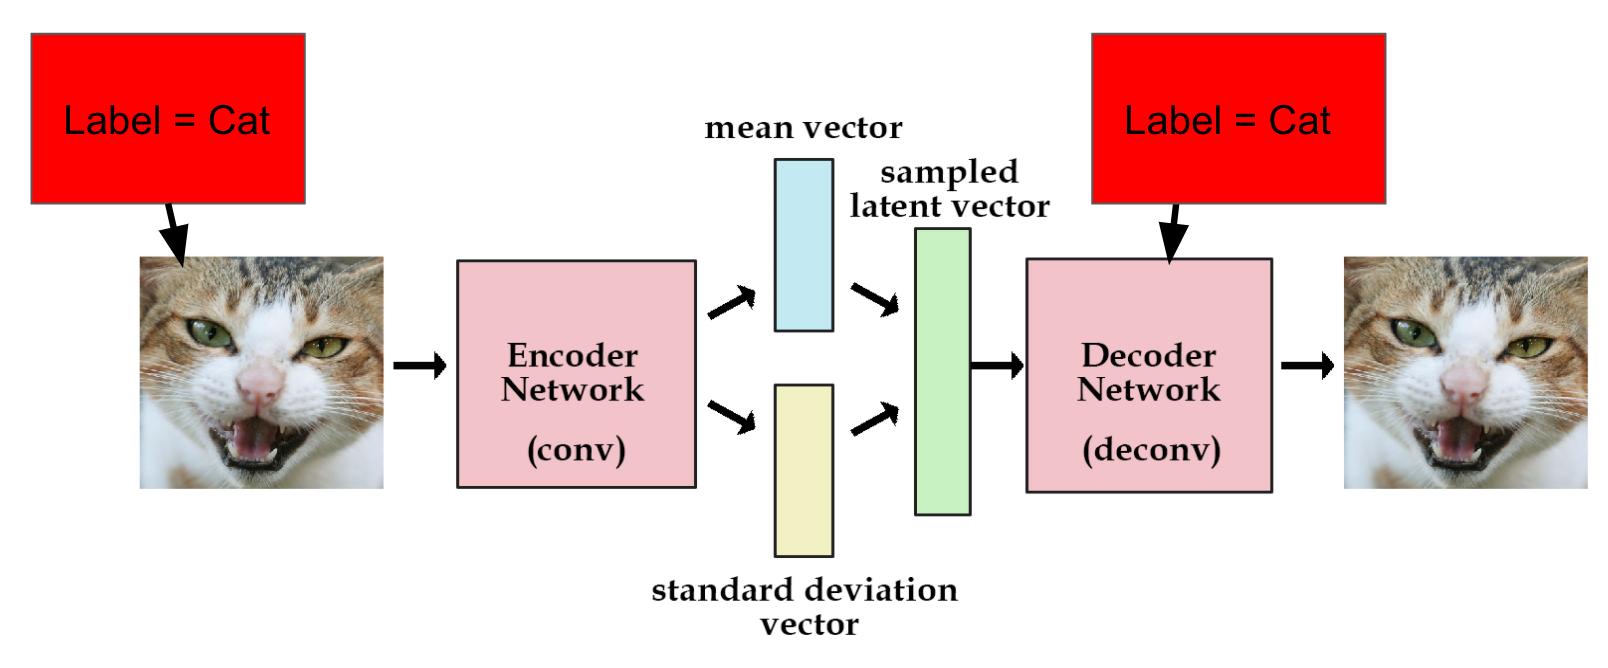
\includegraphics[width=0.9\textwidth]{images/cvae_simple.png}
\centering
\end{minipage}


%\begin{minipage}[b]{\textwidth}
%\center
%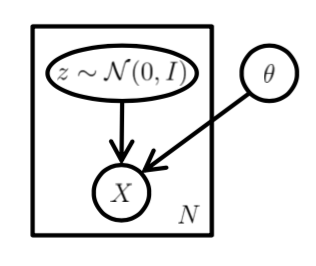
\includegraphics[width=0.45\textwidth]{images/graphical_model.png}
%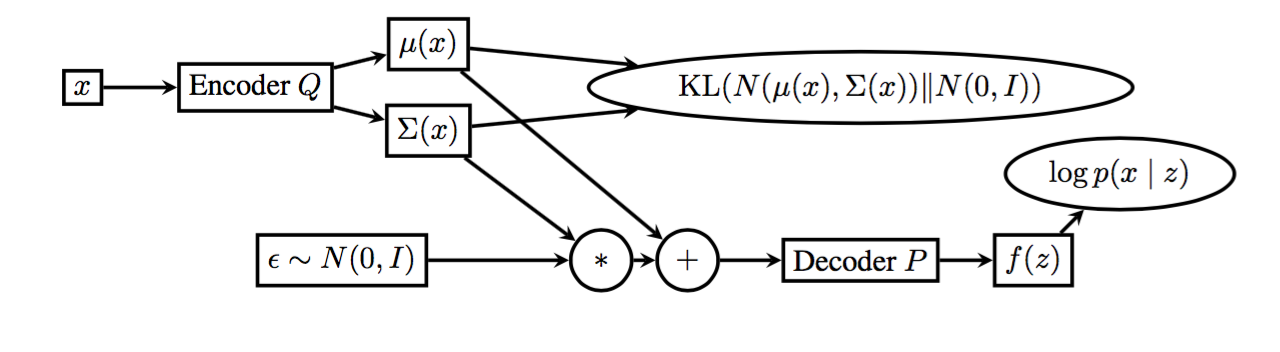
\includegraphics[width=0.9\textwidth]{images/vae2.png}
%\centering
%\end{minipage}
%\begin{equation}
%\log p(x)
%\ge \E_{z \sim Q(\cdot \mid x)}[\log p(x \mid z)]
%- \op{KL}(Q(z \mid x) \| p(z)).
%\end{equation}
%\begin{minipage}[b]{\textwidth}
%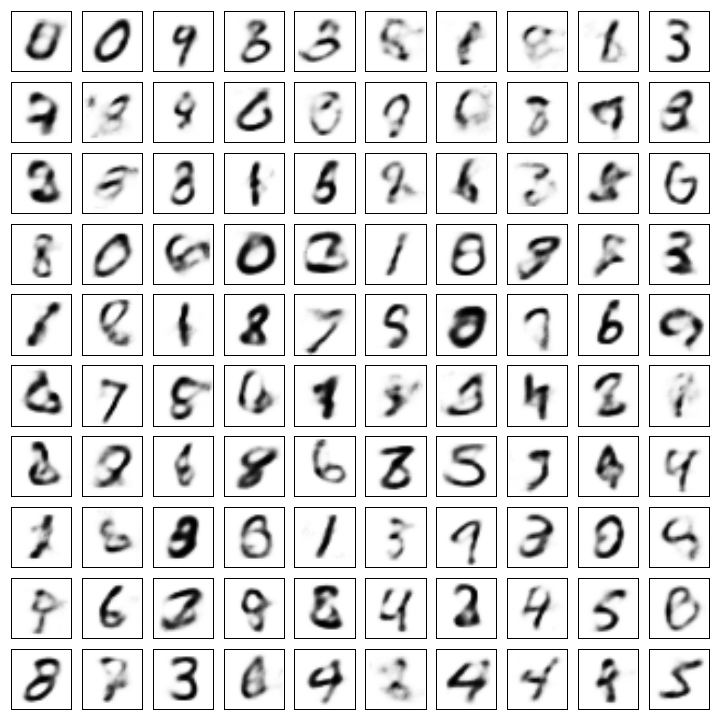
\includegraphics[width=0.48\textwidth]{images/vae_images.png}
%\centering
%\end{minipage}
}

%\headerbox{Conditional VAE (CVAE)}{name=CVAE,column=0,below=VAE}{
%\begin{itemize}\compresslist
%\item condition everything on label $y$
%\end{itemize}
%\begin{minipage}[b]{\textwidth}
%\center
%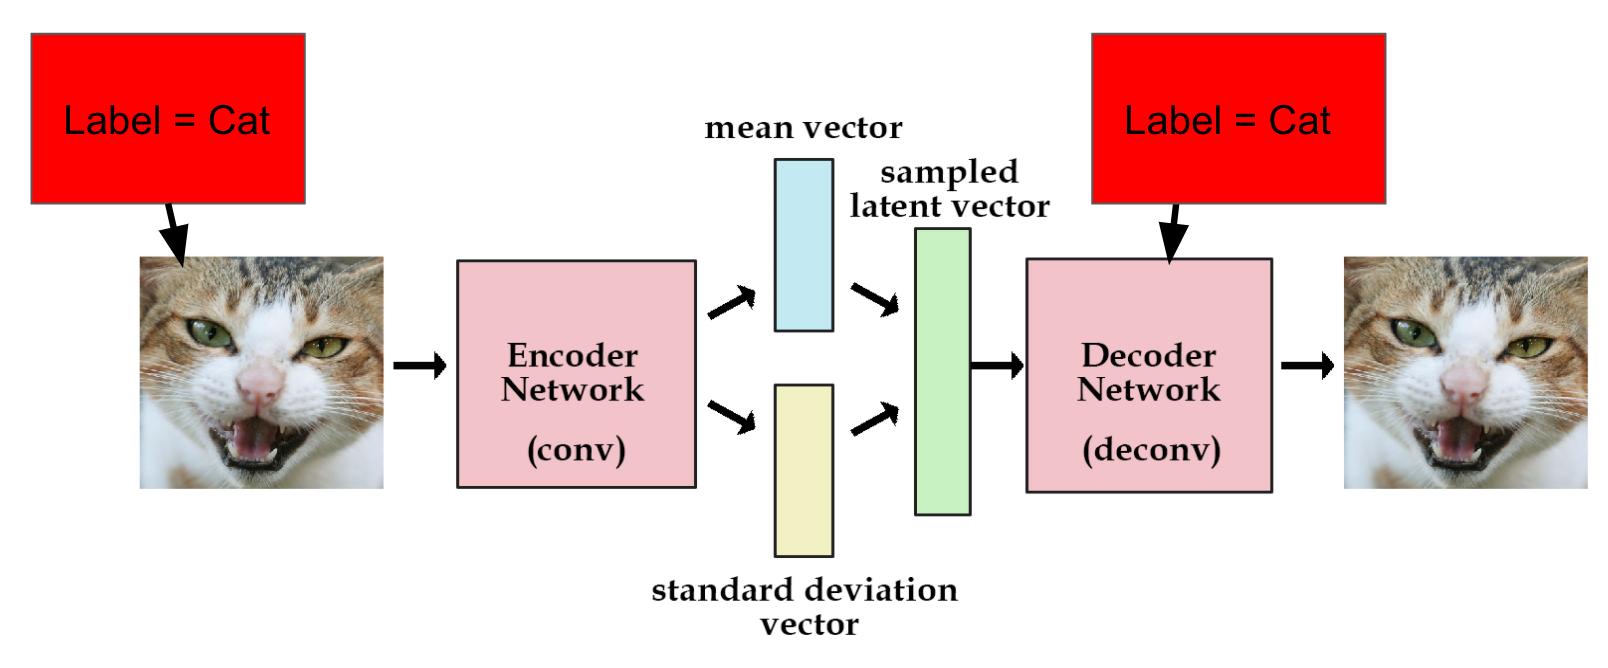
\includegraphics[width=0.9\textwidth]{images/cvae_simple.png}
%\centering
%\end{minipage}
%\begin{scriptsize}
%\begin{equation}
%\log p(x \mid y)
%\ge \E_{z \sim Q(\cdot \mid y,x)}[\log p(x \mid y,z)]
%- \op{KL}(Q(z \mid x,y) \| p(z \mid y)).
%\end{equation}
%\end{scriptsize}
%\begin{minipage}[b]{\textwidth}
%\center
%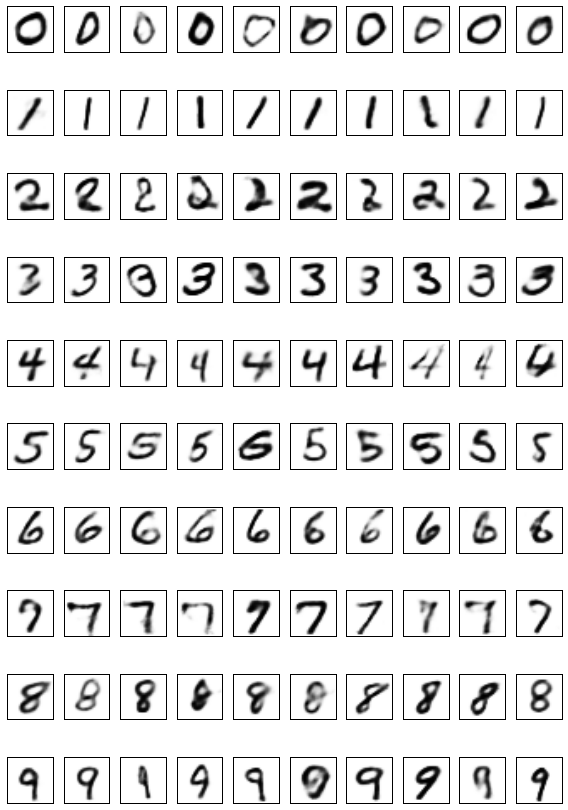
\includegraphics[width=0.48\textwidth]{images/cvae_images.png}
%\centering
%\end{minipage}
%}

\headerbox{CVAE for image completion}{name=completion,column=0,below=VAE}{ % This block's bottom aligns with the bottom of the conclusion block
Generator receives half the image, generates the rest

\begin{minipage}[b]{\textwidth}
\center
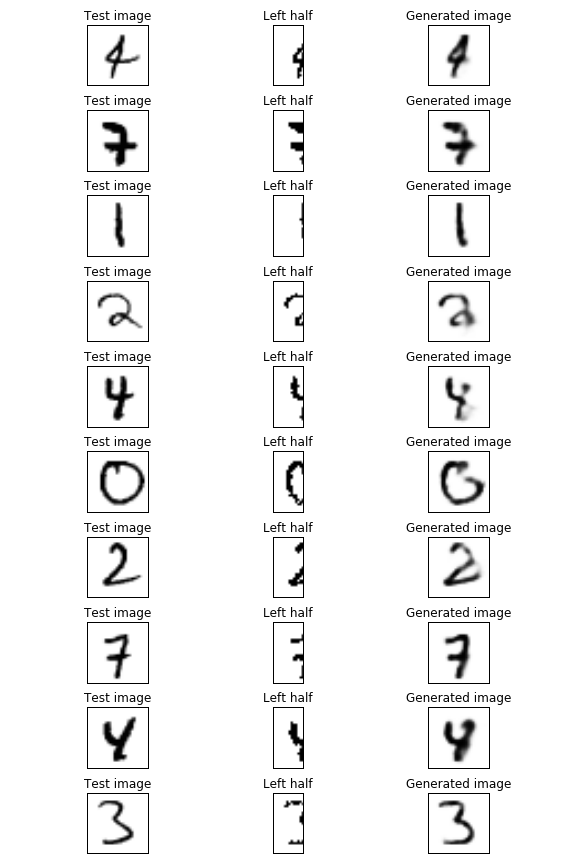
\includegraphics[width=0.48\textwidth]{images/left_half.png}
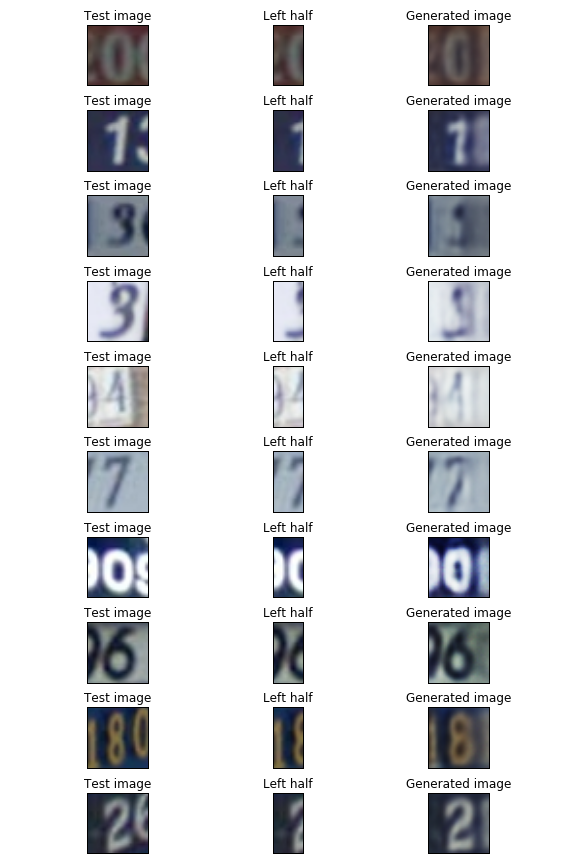
\includegraphics[width=0.48\textwidth]{images/svhn_left_half.png}
\centering
\end{minipage}


}

\headerbox{CVAE for style transfer}{name=style,column=0,below=completion}{ % This block's bottom aligns with the bottom of the conclusion block
Transferring the style of the first column to all digits

\begin{minipage}[b]{\textwidth}
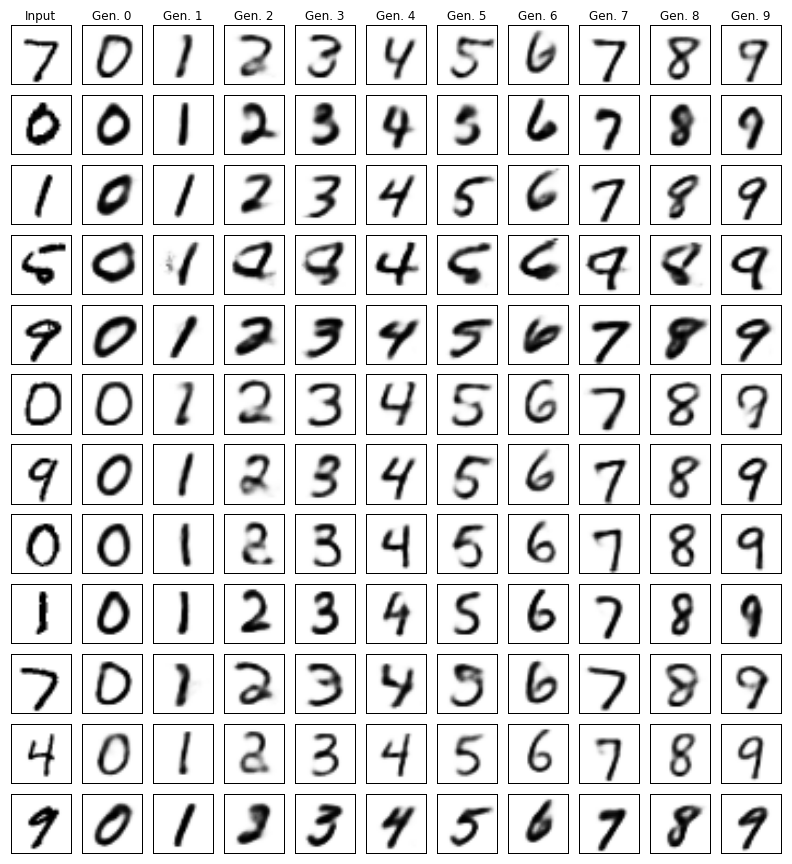
\includegraphics[width=0.48\textwidth]{images/style.png}
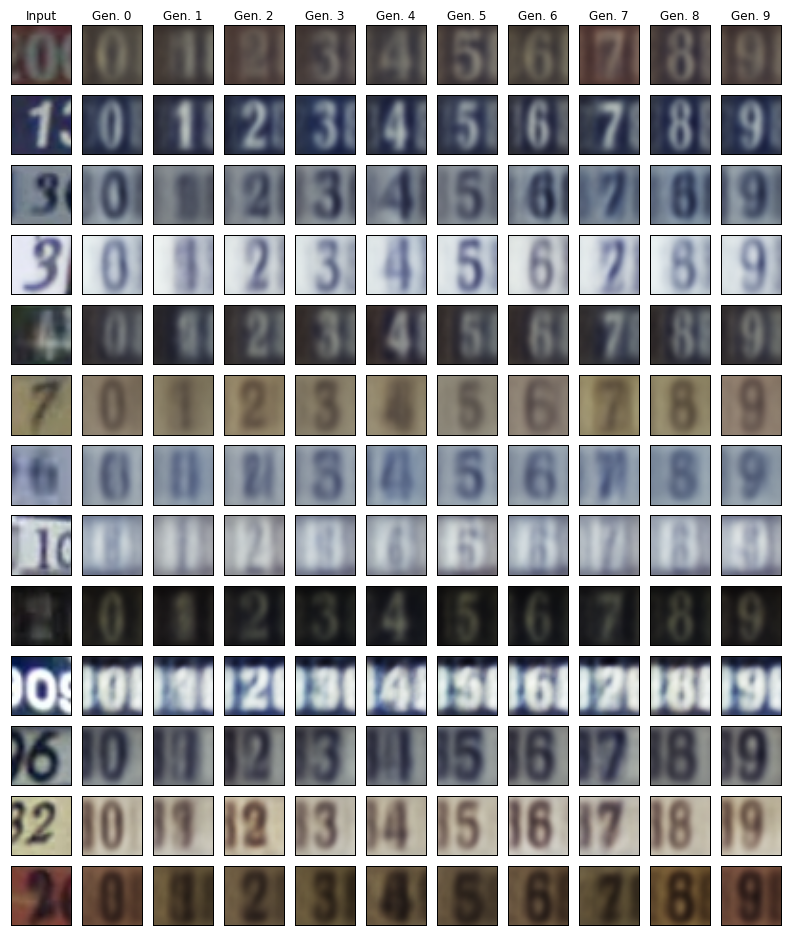
\includegraphics[width=0.46\textwidth]{images/svhn_cvae_fc_style.png}
\centering
\end{minipage}
}











\headerbox{Adding GANs}{name=gan,row=0, column=1}{ % This block is as tall as the references
\begin{itemize}\compresslist
    \item Add discriminator $D$ to encourage sharpness
    \item   Replace the pixel-wise VAE reconstruction loss by learned feature representations in GAN discriminator. \cite{larsen2015autoencoding}
    \item Objective for the generator (VAE) $G$:
    $$
    \mathcal{L} = \mathcal{L}_{\textit{prior}} + \mathcal{L}_{\textit{REC}} + \mathcal{L}_{\textit{GAN}},
    $$
    where
    %\begin{scriptsize}
    \begin{align}
    \mathcal{L}_{\textit{prior}}& =  KL(p_z(z),q(z|x)),\\
    \mathcal{L}_{\textit{REC}} &= -\mathbb{E}_{q(Z|X)}[p(\textit{Dis}_l(X)|Z)],\\
    \mathcal{L}_{\textit{GAN}} &= -\mathbb{E}_{z\sim p_z(z)}[\log  D(G(z))].
    \end{align}
    %\end{scriptsize}
    \item Objective for the discriminator $D$:
    $$
    -\mathbb{E}_{x\sim p_{\textit{data}}}[\log D(x)] - \mathbb{E}_{z\sim p_z(z)}[\log (1 - D(G(z)))].
    $$
\item In our implementations we use the DCGAN architecture \cite{radford2015unsupervised}
\end{itemize}



%\begin{minipage}[b]{\textwidth}
%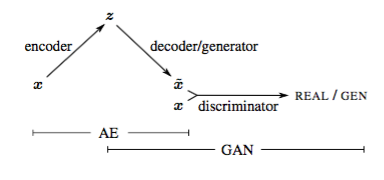
\includegraphics[width=0.8\textwidth]{images/vaegan.png}
%\centering
%\end{minipage}



\begin{minipage}[b]{\textwidth}
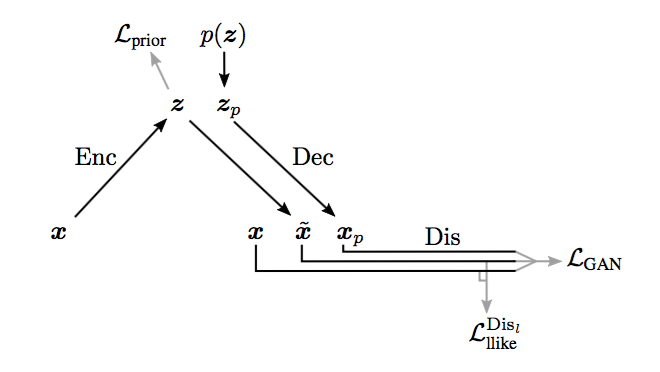
\includegraphics[width=0.6\textwidth]{images/vaegan2.png}
\centering
\end{minipage}

Generated output of VAE with GAN (right) and without (left).

\begin{minipage}[b]{\textwidth}
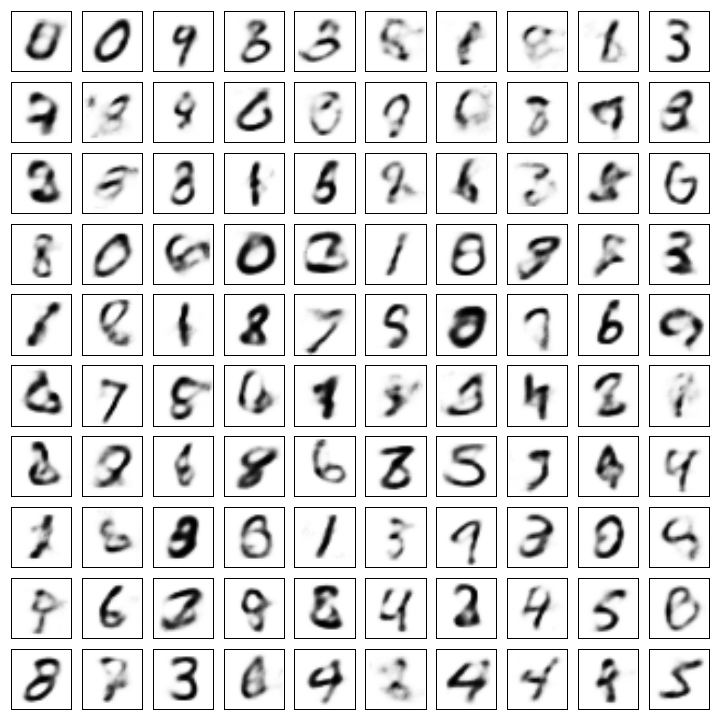
\includegraphics[height=2in]{images/vae_images.png}
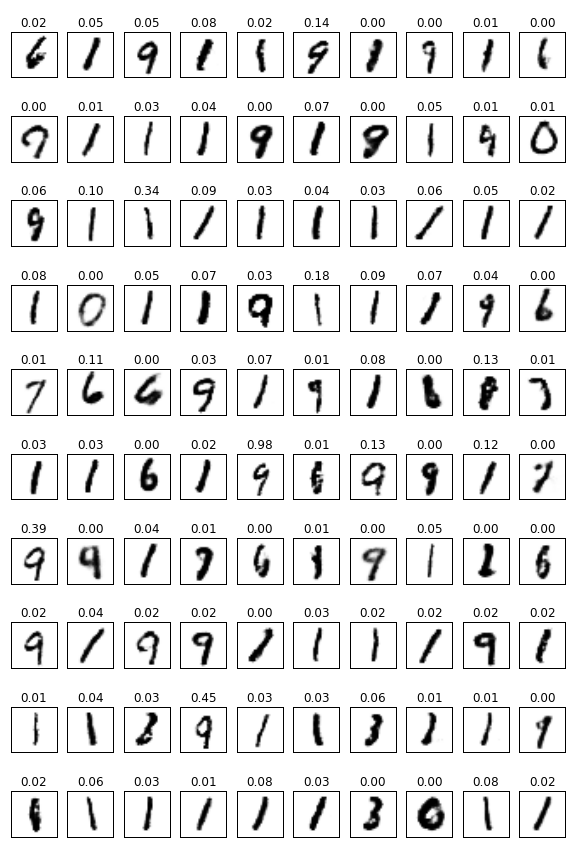
\includegraphics[height=2in]{images/VAEGAN_gen_conv.png}
\centering
\end{minipage}
%\begin{minipage}[b]{0.4\textwidth}
%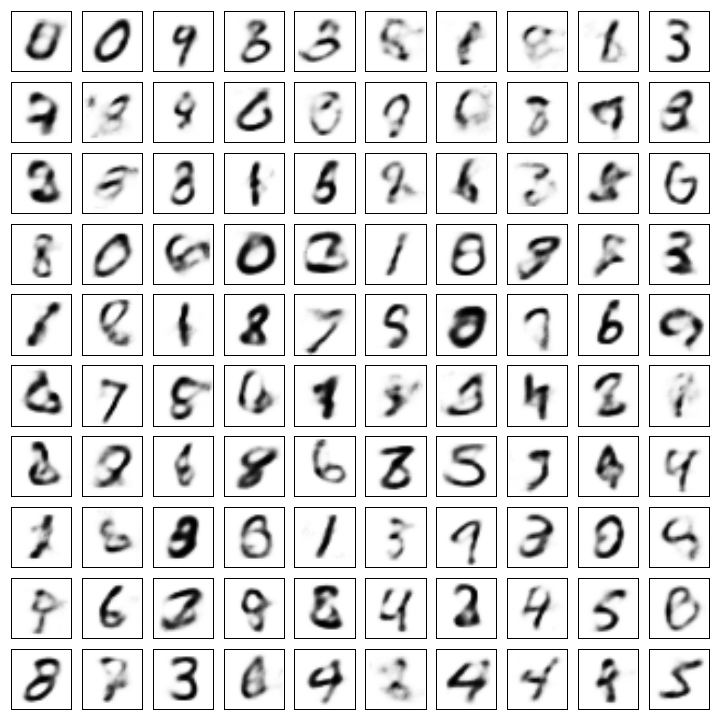
\includegraphics[width=0.48\textwidth]{images/vae_images.png}
%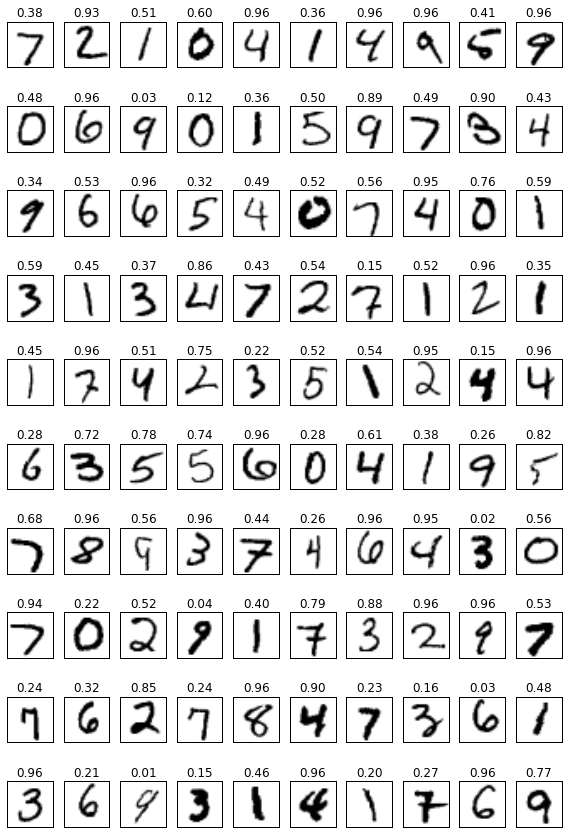
\includegraphics[width=0.4\textwidth]{images/vaegan_images.png}
%\centering
%\end{minipage}
}




\headerbox{CVAE with CGAN}{name=cvaegan,column=1,below=gan}{
\begin{itemize}\compresslist
 \item Add a conditional GAN on top of a conditional VAE.
    \item A conditional GAN has a discriminator assigning probability to real images with different labels and fake images as a single class respectively.
   \cite{mirza2014conditional}
\end{itemize}
%\begin{minipage}[b]{\textwidth}
%\includegraphics[width=0.8\textwidth]{images/cvaegan_structure.png}
%\centering
%\end{minipage}
%\begin{minipage}[b]{\textwidth}
%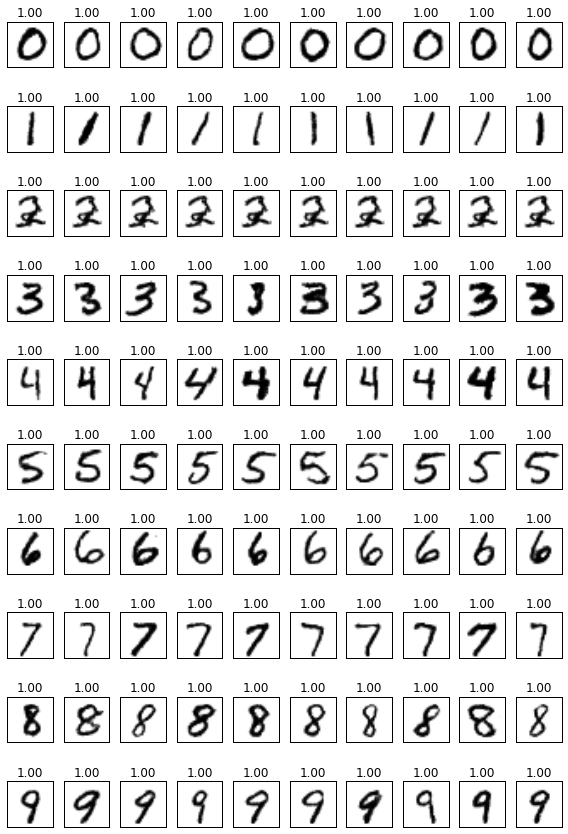
\includegraphics[width=0.45\textwidth]{images/cvaegan_images1.png}
%\centering
%\end{minipage}
%\begin{minipage}[b]{\textwidth}
%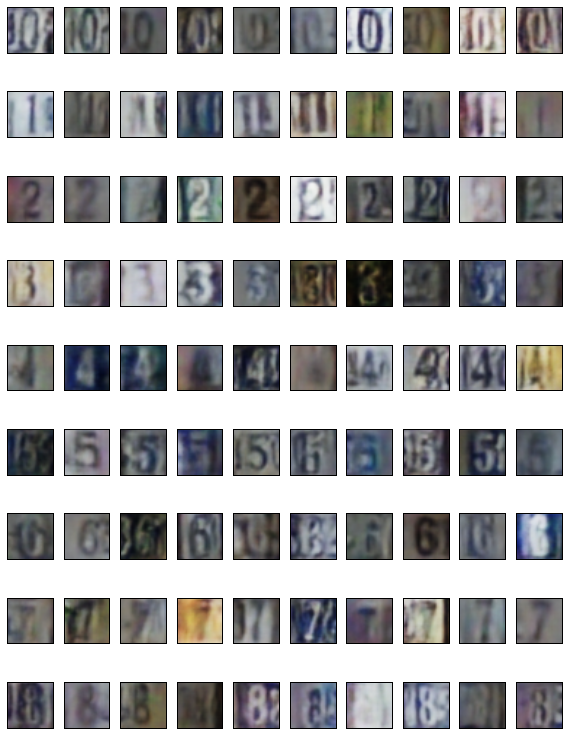
\includegraphics[width=0.45\textwidth]{images/cvaegan_images2.png}
%\centering
%\end{minipage}

\begin{minipage}[b]{\textwidth}
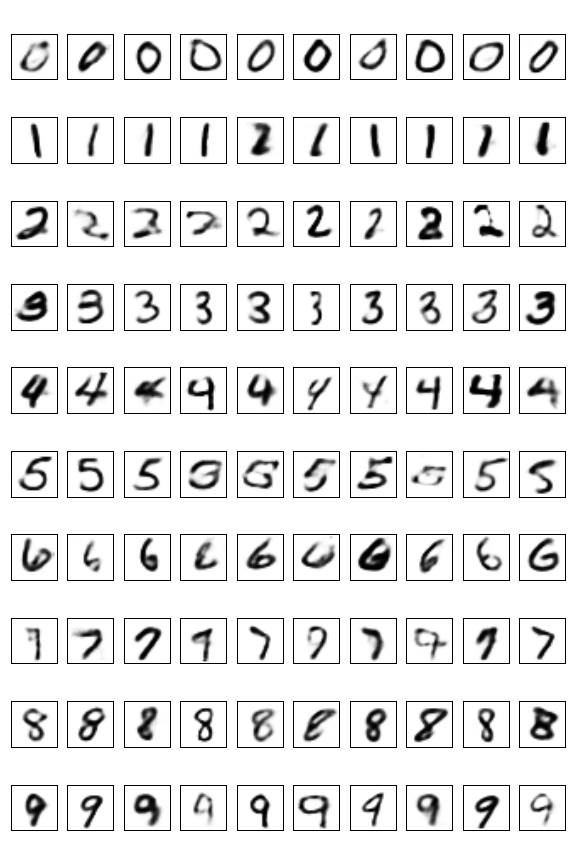
\includegraphics[height=2.2in]{images/by_label.png}
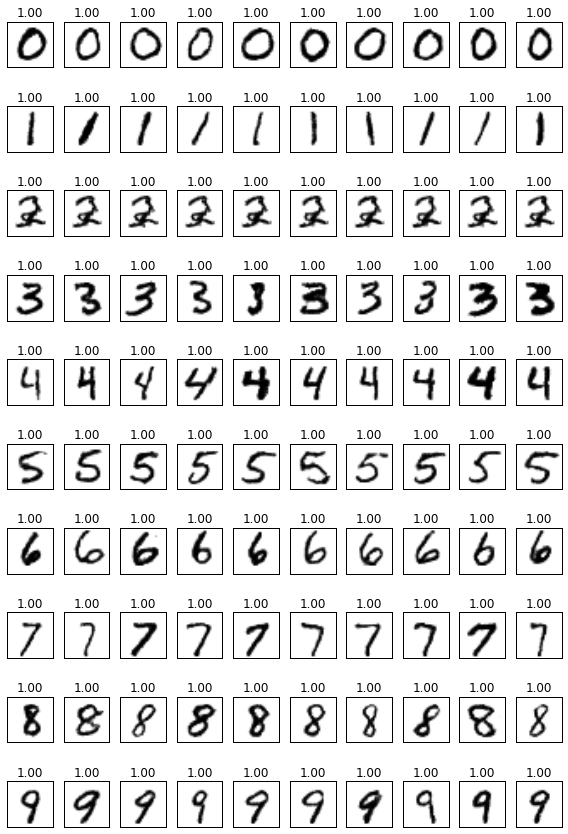
\includegraphics[height=2.2in]{images/cvaegan_images1.png}
\centering
\end{minipage}

\begin{minipage}[b]{\textwidth}
\center
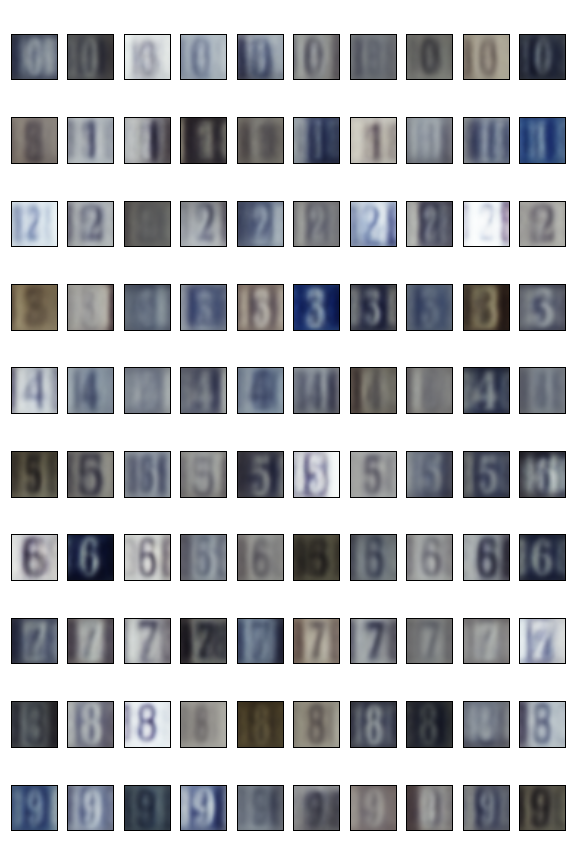
\includegraphics[height=2.2in]{images/svhn_cvae_fc_label_gen.png}
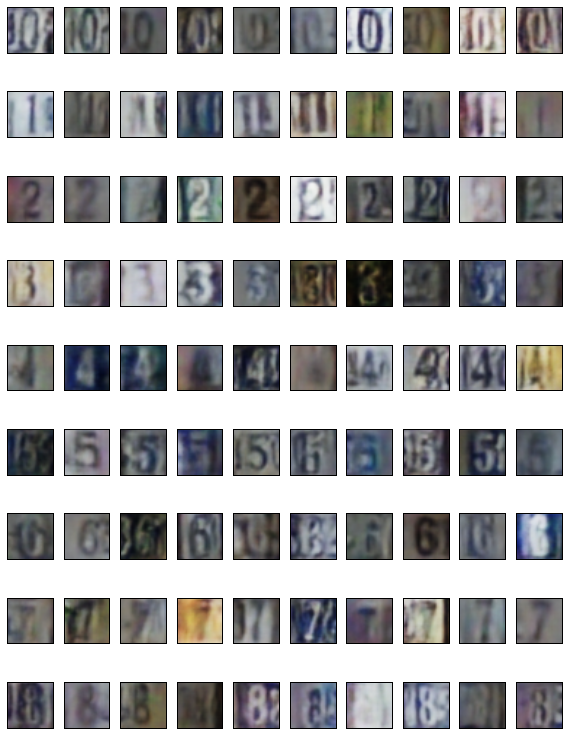
\includegraphics[height=2.2in]{images/cvaegan_images2.png}
\centering
\end{minipage}
}

\headerbox{Semi-supervised learning (SSL) VAE}{name=ssl,column=2, row=0}{
\begin{itemize}\compresslist
    \item Handle datasets with missing labels
    \item Models label distribution
    \item Labeled and unlabeled examples enter loss differently: see $\mathcal{L}(x,y)$ and $\mathcal{U}(x)$ below
    \item Use the encoder as a classifier.
\end{itemize}
Labeled and unlabeled loss, respectively:
\begin{small}
\begin{align}
\log p(x,y)
&\ge \E_{z \sim Q(z \mid x,y)}[\log p(x \mid y,z) + \log p(y)]\\
&\qquad - \op{KL}(Q(z \mid x,y) \| p(z)) =: - \mathcal{L}(x,y)\\
\log p(x) &\ge \sum_y q(y \mid x) (-\mathcal{L}(x,y)) + H(q(y \mid x)) =: -\mathcal{U}(x).
\end{align}
\end{small}

\begin{center}
Validation/test error on MNIST
(55000 training examples)

\begin{tabular}{c|r|r}
& 1000 labeled & 600 labeled\\ \hline
Fully connected & 4.7\%/ 5.1\% & 11.5\%/12.0\%\\
Convolutional & 4.2\%/4.8\% & 6.0\%/6.2\%\\
Kingma et al. \cite{kingma2014semi}
& 2.4\% & 2.6\%
\end{tabular}
\end{center}
%\begin{minipage}[b]{\textwidth}
%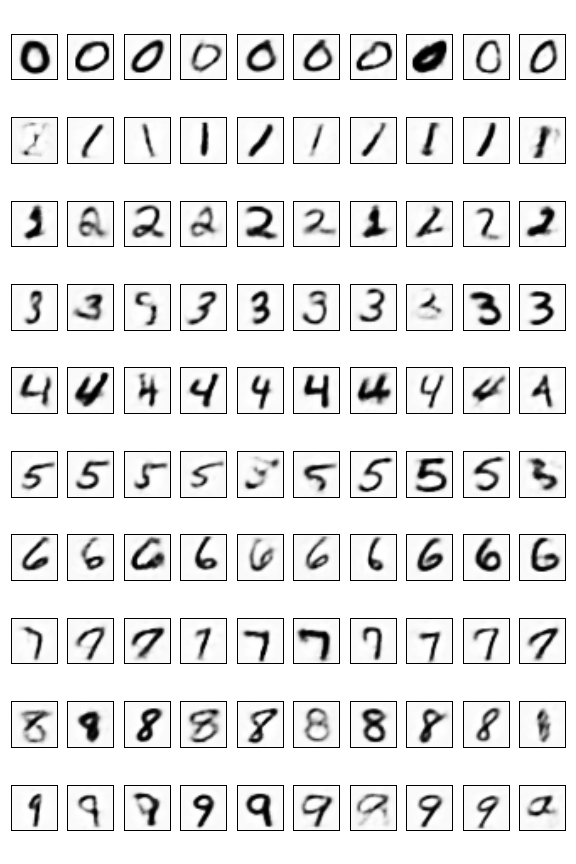
\includegraphics[width=0.5\textwidth]{images/SSL_generate_conv_1000.png}
%\centering
%\end{minipage}
}

\headerbox{SSL with GANs}{name=sslgan,column=2,below=ssl}{
\begin{itemize}\compresslist
 \item Add a conditional GAN on top of a SSL VAE.
 \item Both the discriminator of CGAN and the encoder of SSL VAE can be used as a classifier. We used the latter.
 \item Performance: Currently similar to SSL VAE.
\end{itemize}
%\begin{minipage}[b]{\textwidth}
%\includegraphics[width=0.8\textwidth]{images/sslgan_structure.png}
%\centering
%\end{minipage}
}

\headerbox{DRAW}{name=DRAW,column = 2, below=sslgan}{
\begin{itemize}\compresslist
\item Attention-based sequential generation
\item RNN structure
\item Generalization 1: Condition DRAW on labels (output appears below).
\item Generalization 2: Taking DRAW as a black-box VAE, add GAN on top of it.

\end{itemize}
\begin{minipage}[b]{\textwidth}
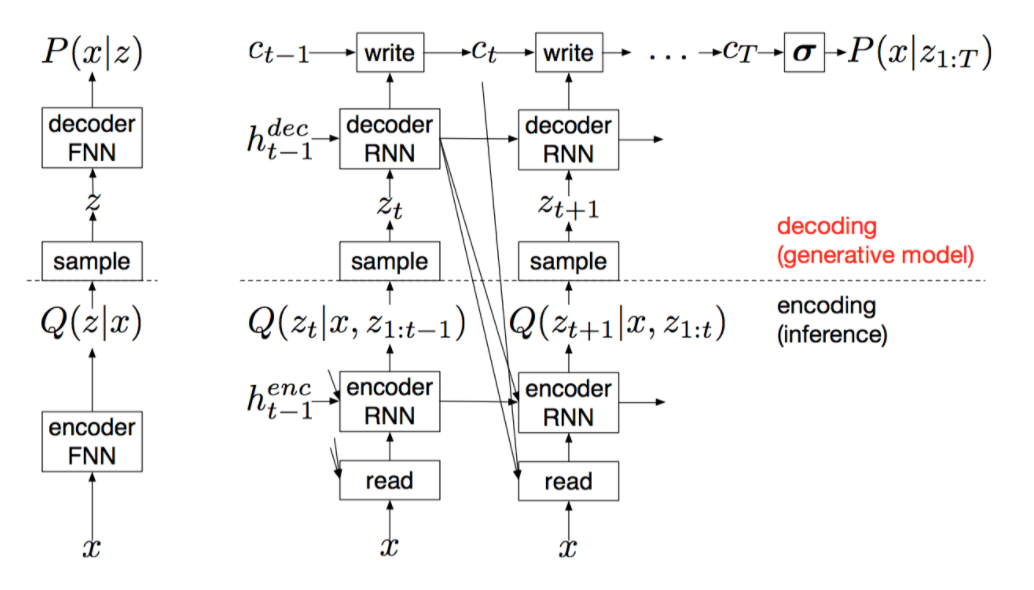
\includegraphics[width=0.6\textwidth]{images/draw_model.png}
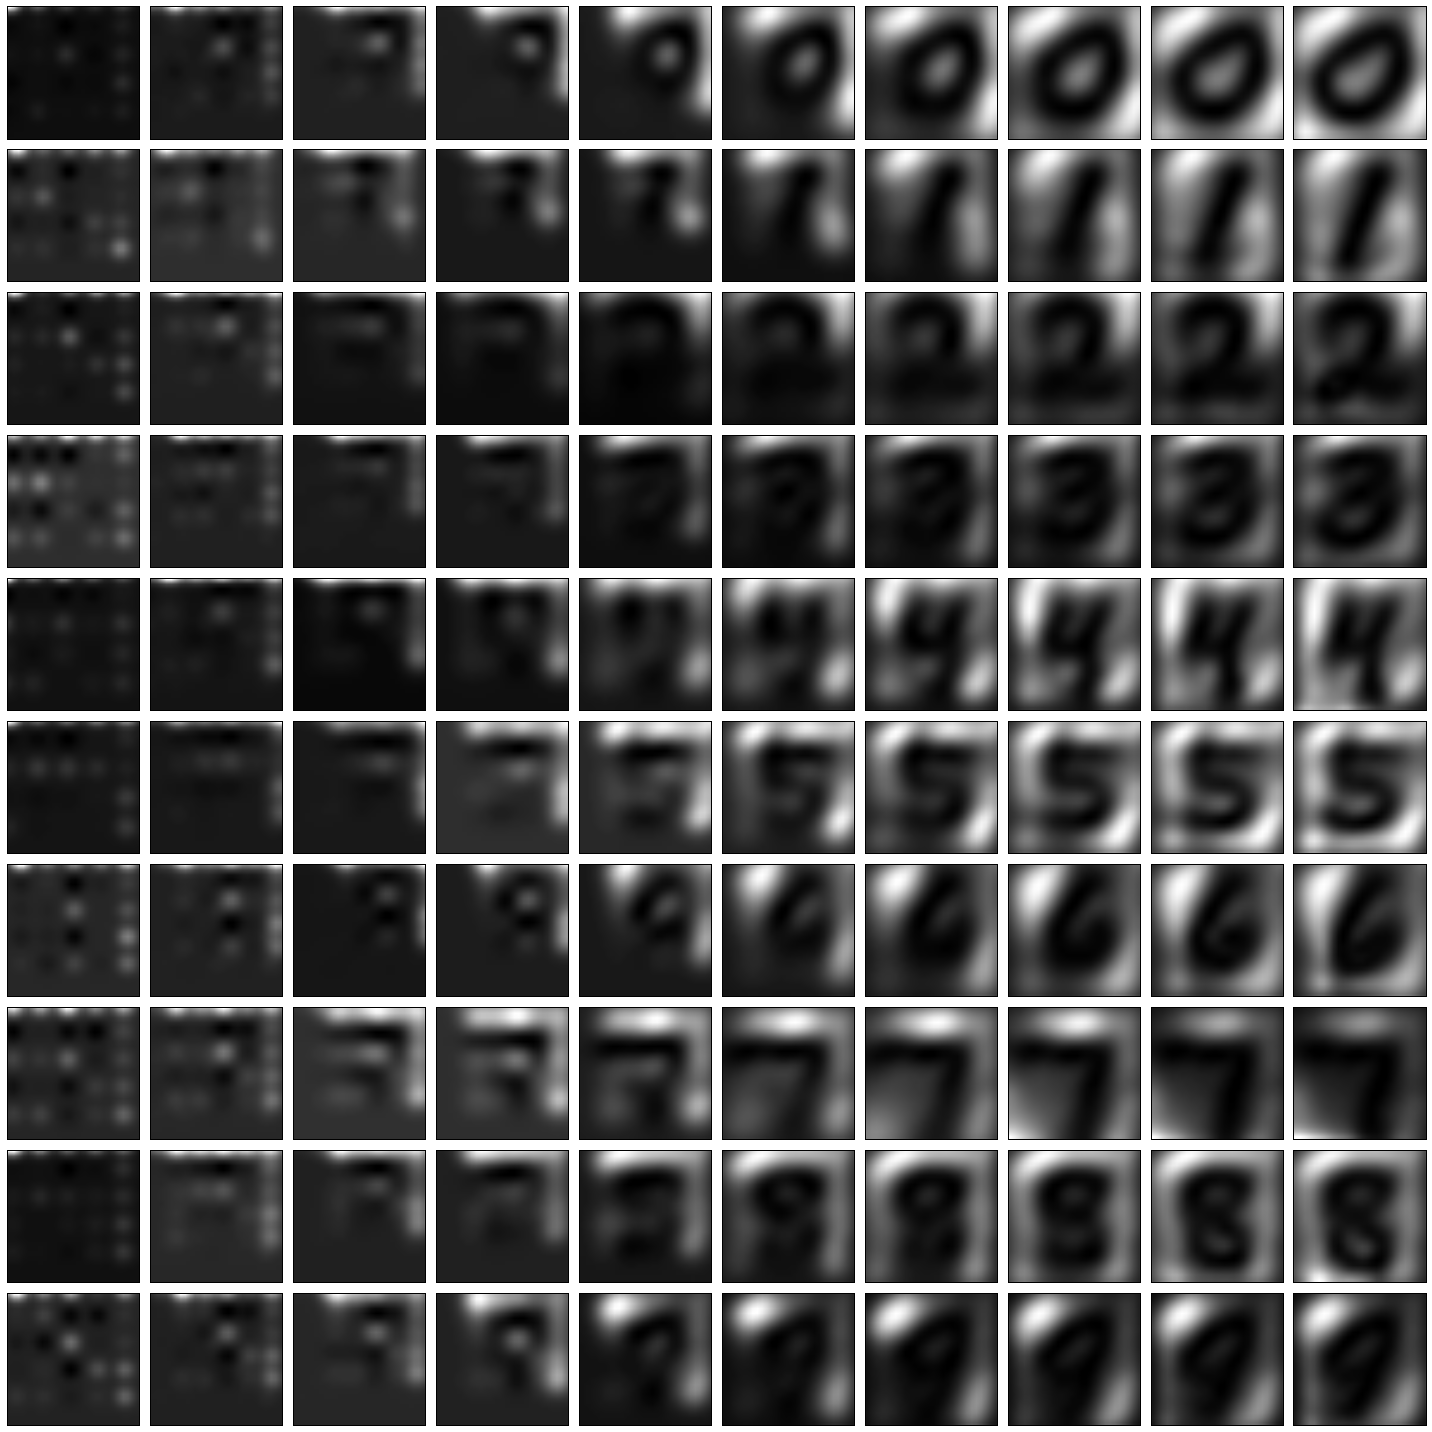
\includegraphics[width=0.38\textwidth]{images/cdraw.png}
\centering
\end{minipage}
}

%\headerbox{DRAW with GANs}{name=drawgan,column=2,below=cvaegan}{
%\begin{itemize}\compresslist
%    \item Add GAN on the top of the last output of DRAW
%\end{itemize}


%\begin{minipage}[b]{\textwidth}
%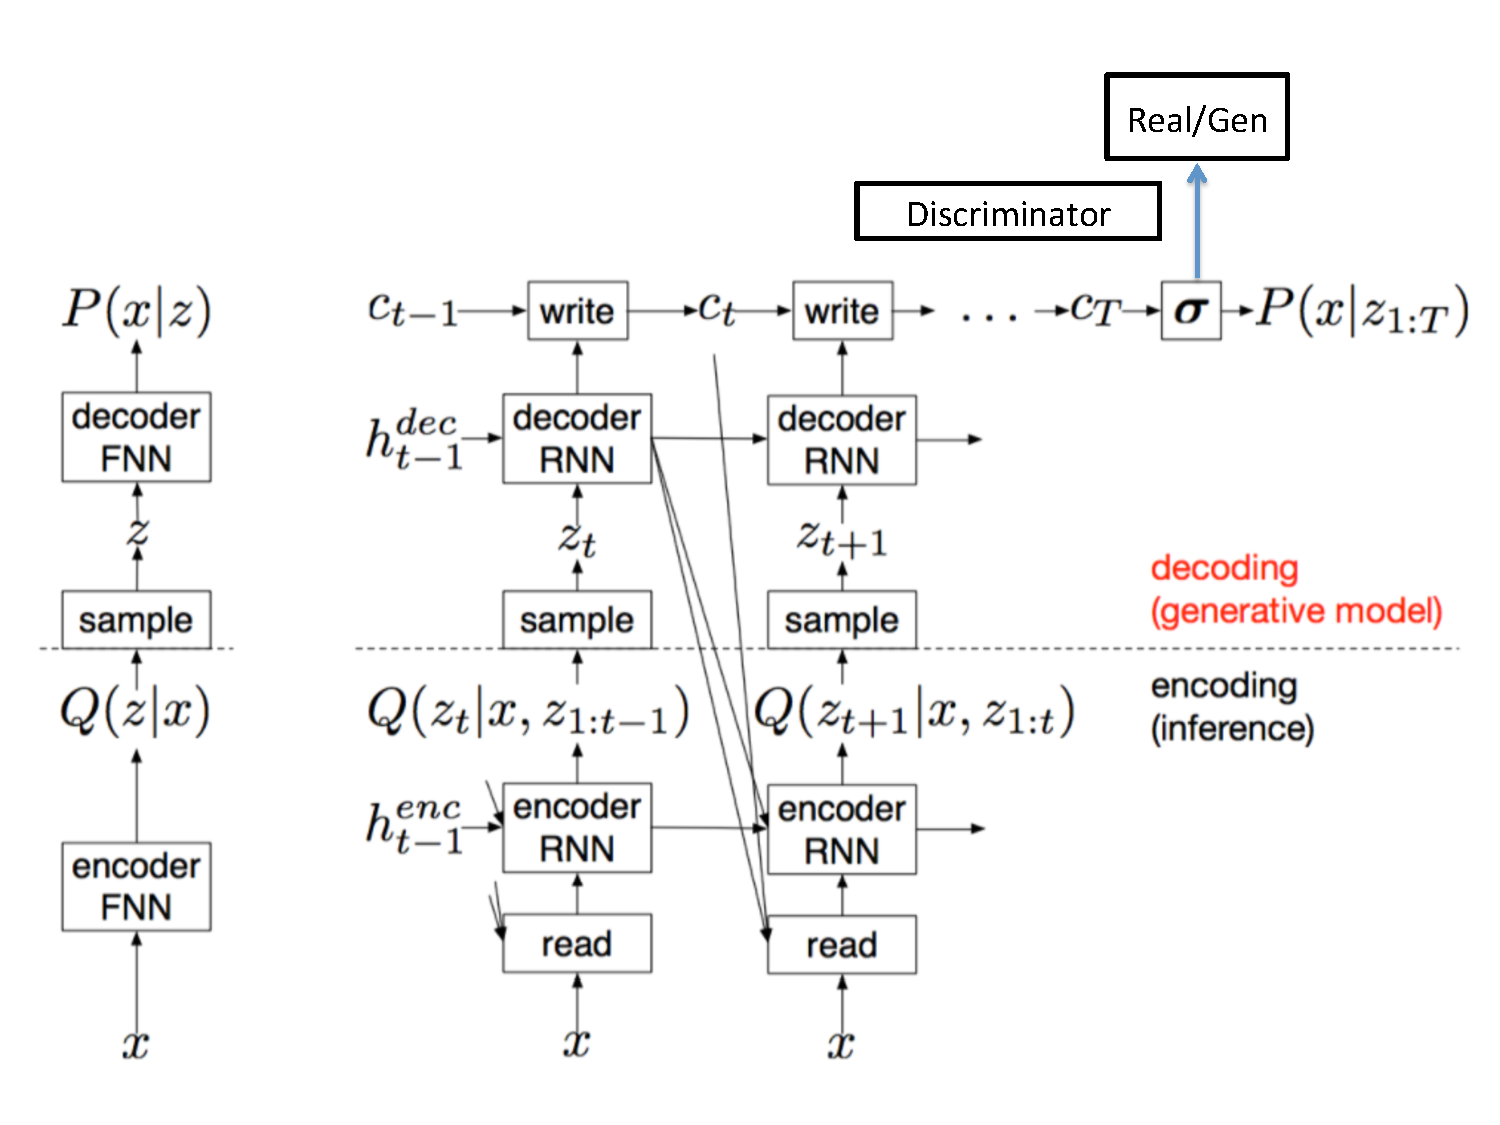
\includegraphics[width=0.8\textwidth]{images/draw_gan.pdf}
%\centering
%\end{minipage}
%}








\headerbox{Future Directions}{name=future,column=2, below=DRAW}{ % This block is as tall as the references block
%a
\begin{itemize}\compresslist
\item Improve our GAN-based models for
\begin{itemize}
\item VAE (generating more diverse digits)
\item SSL (better classification accuracy)
\item DRAW (better generation)
\end{itemize}
\item Consider alternate classifiers for SSL with GAN: encoder, discriminator, or some ensemble?
\item Investigate assessment of generative models.
\end{itemize}
}
 % This block is as tall as the references block
%Autoencoding beyond pixels using a learned similarity metric

%conditional gan

%draw

%\vspace{0.3em}



\renewcommand{\section}[2]{}% removes extraneous ``References'' section title
\headerbox{References}{name=reference,column=2,span=1,below=future}{ % This block is as tall as the references block
\begin{footnotesize}
\bibliographystyle{plain}
\bibliography{cs294_bib}
\nocite{kingma2013auto,kingma2014semi,gregor2015draw,larsen2015autoencoding,doersch2016tutorial,radford2015unsupervised,sohn2015learning}
\end{footnotesize}
}


%----------------------------------------------------------------------------------------
%	CONTACT INFORMATION
%----------------------------------------------------------------------------------------

%----------------------------------------------------------------------------------------
%	CONCLUSION
%----------------------------------------------------------------------------------------


%----------------------------------------------------------------------------------------
%	MATERIALS AND METHODS
%----------------------------------------------------------------------------------------
----------------------------------------------------------------
%	RESUL
%----------------------------------------------------------------------------------------

\end{poster}

\end{document}
